\documentclass{article}[12pt]
% The preceding line is only needed to identify funding in the first footnote. If that is unneeded, please comment it out.
\usepackage{cite}
\usepackage{amsmath,amssymb,amsfonts}
\usepackage{algorithmic}
\usepackage{graphicx}
\usepackage{textcomp}
\usepackage{hyperref}
\usepackage{physics}
\usepackage{mathtools}
\usepackage{comment}
\newcommand{\R}{\mathbb{R}}
\newcommand{\Z}{\mathbb{Z}}
\newcommand{\C}{\mathbb{C}}
\newcommand{\Q}{\mathbb{Q}}

\newcommand{\T}{\mathbb{T}}
\newcommand{\p}{\mathcal{P}}
\newcommand{\N}{\mathbb{N}}
\newcommand{\Hilb}{\mathcal{H}}
\newcommand{\Exp}{\mathbb{E}}
\newcommand{\E}{\mathcal{E}}
\newcommand{\w}{\wedge}\usepackage{xcolor}

\DeclarePairedDelimiter\ceil{\lceil}{\rceil}
\DeclarePairedDelimiter\floor{\lfloor}{\rfloor}

\usepackage{braket}

\renewcommand\bra[1]{{\langle{#1}|}}
\makeatletter
\renewcommand\ket[1]{%
  \@ifnextchar\bra{\k@t{#1}\!}{\k@t{#1}}%
}
\newcommand\k@t[1]{{|{#1}\rangle}}
\makeatother

\def\BibTeX{{\rm B\kern-.05em{\sc i\kern-.025em b}\kern-.08em
    T\kern-.1667em\lower.7ex\hbox{E}\kern-.125emX}}
\begin{document}
\textbf{CS230 Notes} : Soham Joshi
\section{Circuits}

A ciruit is a black box with 
\begin{enumerate}
  \item One or more discrete values input terminals
  \item One or more discrete valued output terminals
  \item Functional specification : reln bw inputs and outputs
  \item Timing sp : Delay bw inputs changing and outputs resp
\end{enumerate}

Difference : 
\begin{enumerate}
  \item Element : small circuit (black box)
  \item Node : wire (input, output, internal)
  \begin{enumerate}
    \item Input : recv values from outside
    \item Output : give values
    \item Internal : Neither of the above two.
  \end{enumerate}
\end{enumerate}

Types of digital circuits :
\begin{enumerate}
  \item Combinational : Outputs depend only on the current values of the inputs, e.g. logic gates :- called memoryless
  \begin{enumerate}
    \item Outputs = f(inputs) :- specification usually via boolean eq (truth table), and K-maps to simplify the expressions 
    \item Timing : lower and upper bound specification (input -> output)
    \item Popular ckt : full adder, $S = A \oplus B \oplus C_{in}$, $C = AB + BC_{in} + AC_{in}$
    \item Single line with slash :- bus (multiple signals)
    \item Rules : interconnected ckt elements st\begin{enumerate}
      \item Each element is Combinational
      \item Every node is either designated to input/exactly one output terminal of ckt element (\verb|FANIN| not allowed)
      \item No cyclic paths
    \end{enumerate}
  \end{enumerate}
  
  \item Sequential ckt : has memory (chapter 3)
  
\end{enumerate} 

\section{Boolean logic}
Literal : var or its complement
Minterm : Product involving all inputs to Function (e.g. for three inputs A,B,C, AB is not a minterm)
Maxterm : Sum involving all inputs of function
Operator precedence : \verb|NOT| $>$ \verb|AND| $>$ \verb|OR|
Canonical form : 
\begin{enumerate}
  \item sum-of-products form : Sum of all minterms where output is true
  \item product-of-sums form : Product of all maxterms where output is false
\end{enumerate}
Boolean algebra : axioms, theorems given below.
\begin{figure}[htbp]
\centerline{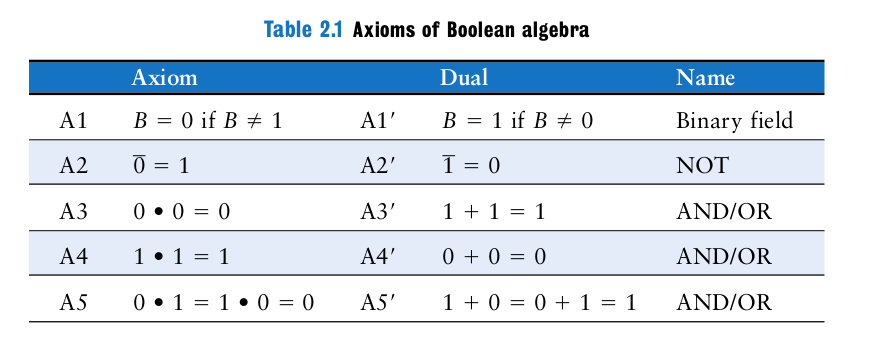
\includegraphics[scale = 0.25]{../Images/a1.png}}
\end{figure}
\begin{figure}[htbp]
\centerline{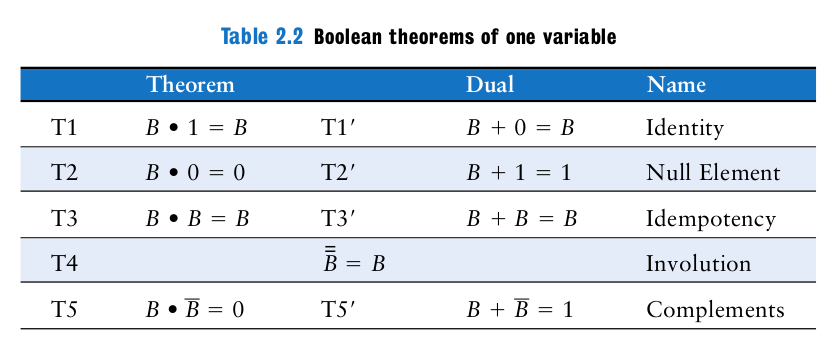
\includegraphics[scale = 0.25]{../Images/a2.png}}
\end{figure}
Theorems of many vars : 
\begin{figure}[htbp]
\centerline{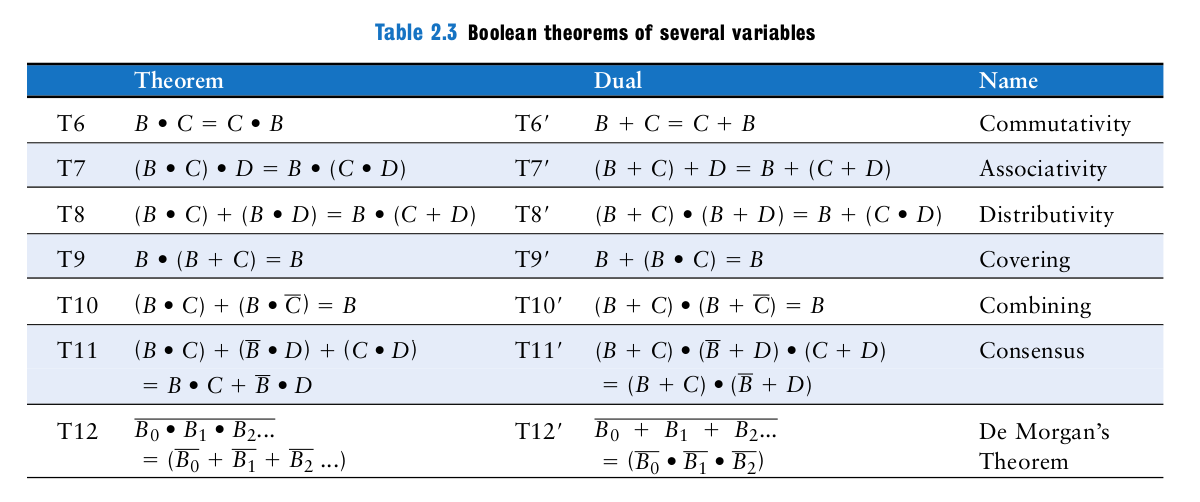
\includegraphics[scale = 0.25]{../Images/a3.png}}
\end{figure}

Proving theorems in boolean algebra : Truth table! \\
Simplifying equations : Use theorems of many vars. \\ 
Minimized formula : Fewest number of implicants. \\
Implicant : Product term in the sum of products representation \\
Prime implicant : Cannot be combined with other implicants to form a new implicant with fewer literals. \\
All implicants in minimal equation must be prime.

Note : Expanding an implicant is sometimes useful in minimization. \\ 
Simplifying reduces the number of gates used to physically
implement the function, thus making it smaller, cheaper, and possibly
faster.
\begin{figure}[htbp]
\centerline{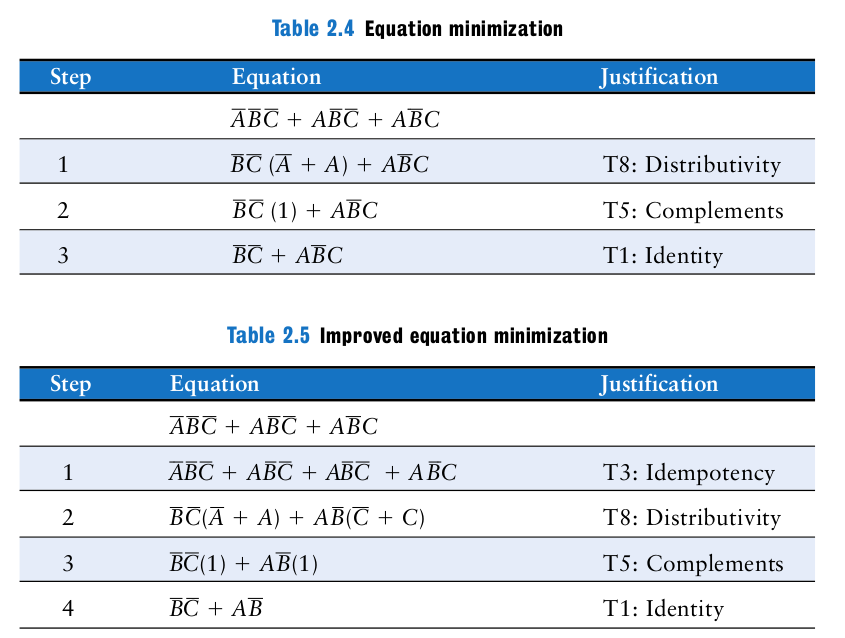
\includegraphics[scale = 0.25]{../Images/impl.png}}
\end{figure}

\section[short]{Gates}

schematic : a diagram of a digital circuit showing the elements and
the wires that connect them together.

Guidelines : 
\begin{enumerate}
  \item Inputs are on the left (or top) side of a schematic.
  \item Outputs are on the right (or bottom) side of a schematic.
  \item Whenever possible, gates should flow from left to right.
  \item Straight wires are better to use than wires with multiple corners
  (jagged wires waste mental effort following the wire rather than
  thinking of what the circuit does).
  \item Wires always connect at a T junction.
  \item A dot where wires cross indicates a connection between the wires.
  \item Wires crossing without a dot make no connection.
\end{enumerate}

This style is called programmable logic array (PLA). \\ 
Example : priority circuit 
\begin{figure}[htbp]
\centerline{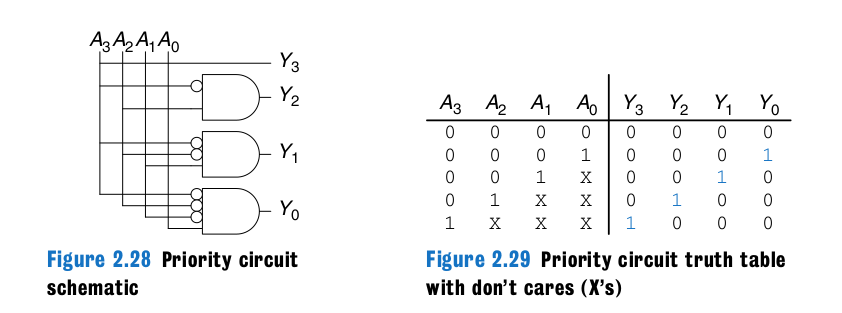
\includegraphics[scale = 0.3]{../Images/priority.png}}
\end{figure}

\section{Multilevel combo logic}
Layer of \verb|AND| followed be level of \verb|OR|. 

Trick : 
\begin{enumerate}
  \item three input XOR = $(A \oplus B) \oplus C$  = two level of XORs.
  \item 8 input XOR = eight input \verb|AND| gates, one 128 \verb|OR| gate. But it needs only 7 XORS.
  \item Moving bubble from the end towards left, adding bubbles at input and AND to/from OR.
\end{enumerate}

Special symbols : 
\begin{enumerate}
  \item X(contention) : unknown/illegal value. Driven to both 0 and 1 at the same time. (e.g. FANIN with one input 1, other 0)
  \item Z(floating value) : driven by neither 0 nor 1. Misconception : Z is 0 (not true)
\end{enumerate}

Tristate buffer : Active high enable. (1 enables buffer). Has three possible output states. 0 or 1 or Z (Z when the enable is False).
Used in busses that connect multiple input chips.

K-maps : Easy visual way to minimize logic. Use fewest circles to connect all 1s.

\section{Combinational building blocks}
Multiplexer (mux): 
2 : 1 mux :- S, D0, D1. S = i means Di is the output. 
\begin{figure}[htbp]
\centerline{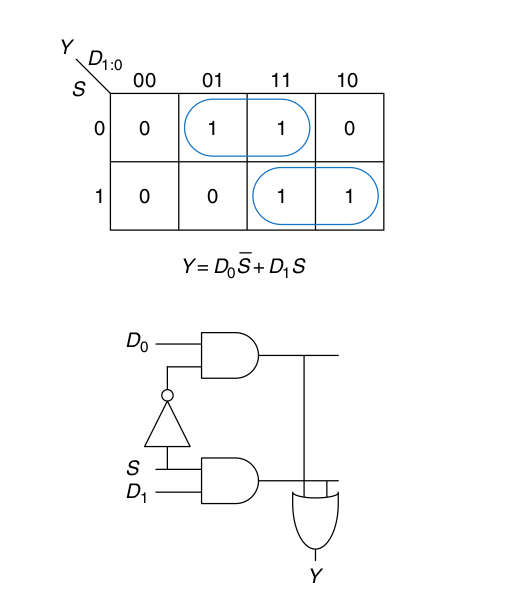
\includegraphics[scale = 0.3]{../Images/mux-21-logic.png}}
\end{figure}
\begin{figure}[htbp]
\centerline{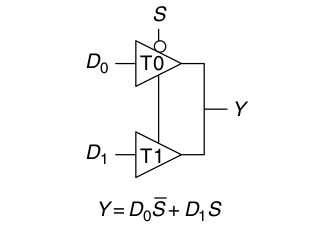
\includegraphics[scale = 0.3]{../Images/mux-21-buff.png}}
\end{figure}

Wider multiplexers :- 4:1 :- two input state signals. \\
N:1 mux :- $log_{2}N$ select lines.
With a little cleverness, we can cut the multiplexer size in half, using
only a $2^N-1$ -input multiplexer to perform any N-input logic function.
The strategy is to provide one of the literals, as well as 0s and 1s, to the
multiplexer data inputs. First layer two 2:1 mux, second layer, one 2:1 mux. (hierarchial)

Decoders : \\ 
A decoder has N inputs and $2^N$ outputs. It asserts exactly one of its
outputs depending on the input combination. (turns one input 1, rest 0 : "one-hot" outputs.)
\begin{figure}[htbp]
\centerline{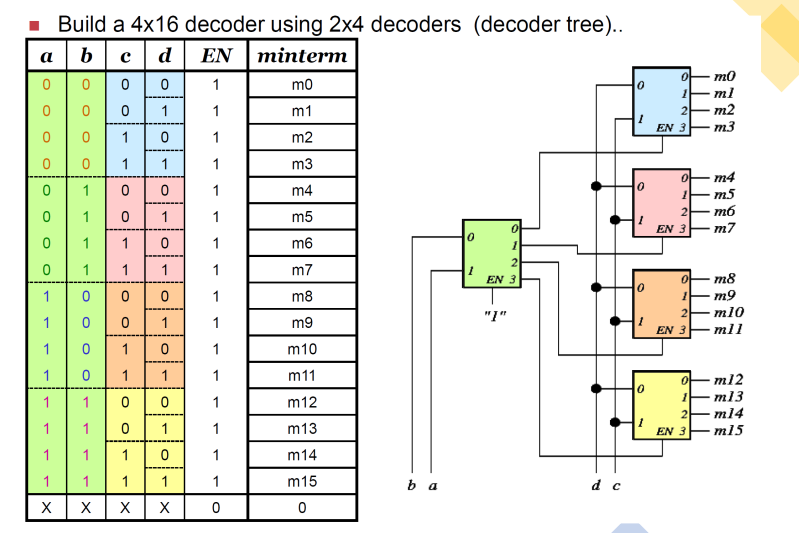
\includegraphics[scale = 0.3]{../Images/dec-tree.png}}
\end{figure}

\section{Sequential Logic Design}
Value depends on current state-variables. Design via finite-state machines. \\ 
Lateches and Flip flops : \\
bistable element (two stable states):- 1 bit of information : fundamental building block of memory. No input but two outputs. 
Analysis : take cases as Q = 0, Q = 1. and look for contradictions. i.e. look for stable points.
\begin{figure}[htbp]
\centerline{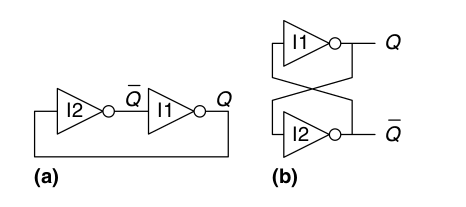
\includegraphics[scale = 0.3]{../Images/mem.png}}
\end{figure}

When power is first applied to a sequential circuit, the initial state is
unknown and usually unpredictable. It may differ each time the circuit is
turned on. Although the cross-coupled inverters can store a bit of information,
they are not practical because the user has no inputs to control the state. \\ 
\textbf{SR Latch} : \\ 
SR latch : two cross coupled NOR gates. The
inputs S and R stand for Set and Reset. To set a bit means to make it
TRUE. To reset a bit means to make it FALSE. The outputs, Q and Q ,
are normally complementary. When R is asserted, Q is reset to 0 and Q
does the opposite. When S is asserted, Q is set to 1 and Q does the
opposite. When neither input is asserted, Q remembers its old value,
Q prev . Asserting both S and R simultaneously doesn't make much sense
because it means the latch should be set and reset at the same time,
which is impossible. The poor confused circuit responds by making both
outputs 0.
\begin{figure}[htbp]
\centerline{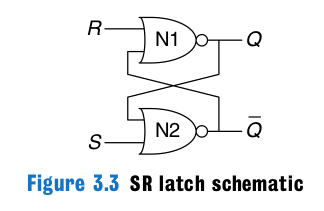
\includegraphics[scale = 0.3]{../Images/sr.png}}
\end{figure}

\begin{figure}[htbp]
\centerline{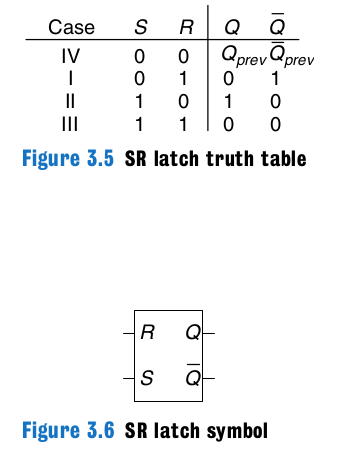
\includegraphics[scale = 0.3]{../Images/sr2.png}}
\end{figure}

No matter what pattern of
setting and resetting occurred in the past, all that is needed to predict
the future behavior of the SR latch is whether it was most recently set
or reset.

\textbf{D Latch} : \\ 
The SR latch is awkward because it behaves strangely when both S and
R are simultaneously asserted. Moreover, the S and R inputs conflate
the issues of what and when. Asserting one of the inputs determines
not only what the state should be but also when it should change.
Designing circuits becomes easier when these questions of what and
when are separated. The D latch in Figure 3.7(a) solves these problems.
It has two inputs. The data input, D, controls what the next state
should be. The clock input, CLK, controls when the state should
change.

\begin{figure}[htbp]
\centerline{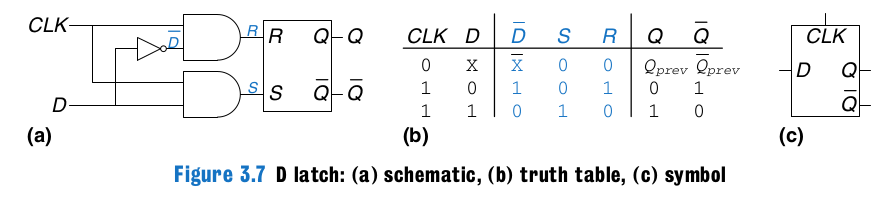
\includegraphics[scale = 0.3]{../Images/d-latch.png}}
\end{figure}

\textbf{D Flip Flop} : 
D flip-flop copies D to Q on the rising edge of the
clock, and remembers its state at all other times.

A D flip-flop is also known as a master-slave flip-flop, an edge-triggered
flip-flop, or a positive edge-triggered flip-flop. The triangle in the symbols
denotes an edge-triggered clock input. The Q output is often omitted when
it is not needed.

\begin{figure}[htbp]
\centerline{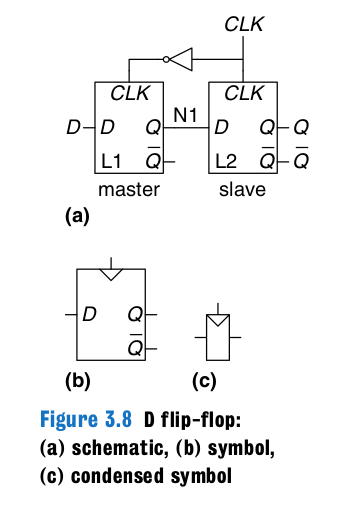
\includegraphics[scale = 0.3]{../Images/d-flip-flop.png}}
\end{figure}

Register : An N-bit register is a bank of N flip-flops that share a common CLK
input, so that all bits of the register are updated at the same time.

Enabled flip-flop : An enabled flip-flop adds another input called EN or ENABLE to
determine whether data is loaded on the clock edge. When EN is
TRUE, the enabled flip-flop behaves like an ordinary D flip-flop.
When EN is FALSE, the enabled flip-flop ignores the clock and
retains its state.

\begin{figure}[htbp]
\centerline{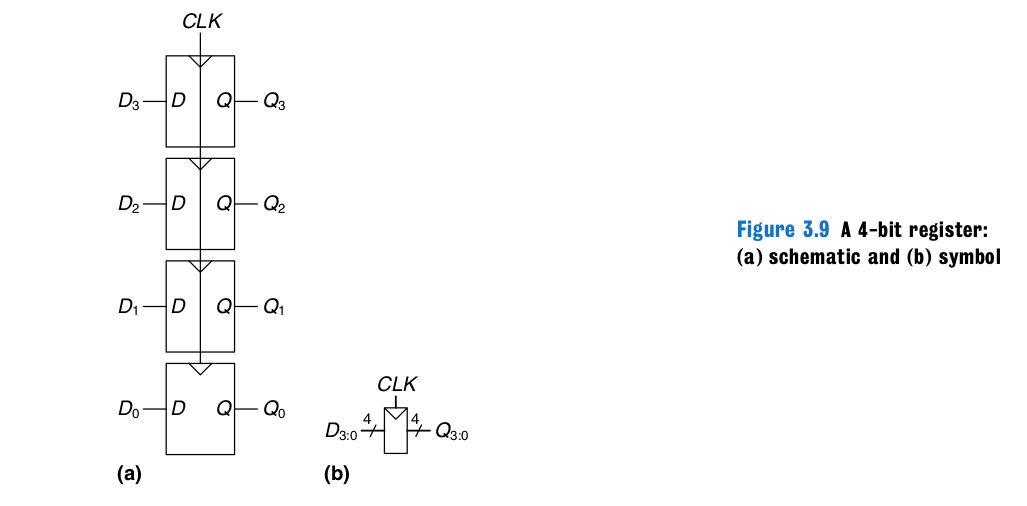
\includegraphics[scale=0.3]{../Images/4-bit-reg.png}}
\end{figure}

\begin{figure}[htbp]
\centerline{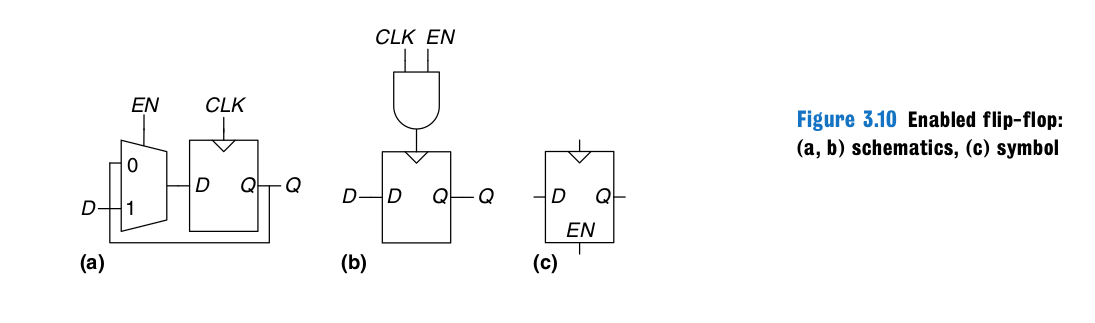
\includegraphics[scale=0.3]{../Images/enabled-flip-flop.png}}
\end{figure}

Resettable flip flops : A resettable flip-flop adds another input called RESET. When RESET
is FALSE, the resettable flip-flop behaves like an ordinary D flip-flop.
When RESET is TRUE, the resettable flip-flop ignores D and resets the
output to 0. Resettable flip-flops are useful when we want to force a
known state (i.e., 0) into all the flip-flops in a system when we first
turn it on.

\subsection{Finite state machines}

\begin{enumerate}
  \item These forms are called finite state machines (FSMs). They get
  their name because a circuit with k registers can be in one of a finite num-
  ber ($2^k$) of unique states.
  \item An FSM has M inputs, N outputs, and k bits of
  state. It also receives a clock and, optionally, a reset signal.
  \item An FSM consists of two blocks of combinational logic, next state logic and output
  logic, and a register that stores the state.
  \item On each clock edge, the FSM advances to the next state, which was computed based on the current state
  and inputs.
  \item There are two general classes of finite state machines, charac-
  terized by their functional specifications. In Moore machines, the outputs
  depend only on the current state of the machine. In Mealy machines, the
  outputs depend on both the current state and the current inputs.
  \item Finite state machines provide a systematic way to design synchronous sequential
  circuits given a functional specification.
\end{enumerate}

General design : 
\begin{enumerate}
  \item For a Moore machine:
  \begin{enumerate}
    \item Write a state transition table.
    \item Write an output table.
  \end{enumerate}
  \item For a Mealy machine:
  \begin{enumerate}
    \item Write a combined state transition and output table.
  \end{enumerate}
  \item Select state encodings--your selection affects the hardware design.
  \item Write Boolean equations for the next state and output logic.
  \item Sketch the circuit schematic.
\end{enumerate}
We will repeatedly use FSMs to design complex digital systems
\end{document}